\documentclass[11pt,a4paper]{article}
\usepackage[utf8]{inputenc}
\usepackage[T1]{fontenc}
\usepackage[spanish]{babel}
\usepackage{lmodern}
\usepackage{amsmath}
\usepackage{graphicx}
\usepackage[margin=2.4cm]{geometry}
\usepackage[hidelinks]{hyperref}
\setlength{\parindent}{0pt}
\setlength{\parskip}{0.5em}
\begin{document}
{\small
\begin{tabular}{@{}l@{}}
\textbf{Matemática Discreta, sección 30} \\
Ivan Morataya --- 16667 \\
David Díaz --- 25314 \\
David Ibaté --- 251732 \\
Miguel Carranza --- 24458 \\
José Ceferino --- 251043
\end{tabular}
}
\section*{Proyecto 4: Calculadora gráfica modular}
\section*{1. Descripción general}
La calculadora permite sumar, restar, multiplicar, dividir y elevar a una
potencia en aritmética modular. También interpreta expresiones con paréntesis.
Se desarrolló en Python con una ventana gráfica de Tkinter, sin dependencias
externas para su funcionamiento.

Trabajar módulo $p$ significa conservar el residuo al dividir entre $p$.
Por ejemplo, $17$ módulo $5$ es $2$, porque $17=3\cdot5+2$. El resultado
siempre se presenta entre $0$ y $p-1$. El programa exige que $p$ sea primo.

\subsection*{Operaciones implementadas}
\begin{itemize}
\item \textbf{Suma, resta y multiplicación:} se realiza la operación y se
conserva su residuo módulo $p$. Por ejemplo, $4-6\equiv3\pmod5$.
\item \textbf{División:} se multiplica por el inverso modular del denominador.
El inverso de $b$ es el número $u$ que cumple $bu\equiv1\pmod p$.
Así, $3/2\equiv3\cdot3\equiv4\pmod5$. No es una división decimal.
Si el denominador es $0$ módulo $p$, la división no existe.
\item \textbf{Potencia:} se calcula el residuo de la potencia sin construir
primero un número enorme. Un exponente negativo utiliza el inverso de la
base; por ejemplo, $2^{-1}\equiv3\pmod5$.
\item \textbf{Agrupación:} los paréntesis indican qué se calcula primero.
Sin ellos, la potencia tiene prioridad, seguida de multiplicación/división
y finalmente suma/resta. Las operaciones de un mismo nivel se realizan de
izquierda a derecha, salvo las potencias encadenadas, que se agrupan a la derecha.
\end{itemize}

\subsection*{Uso de un LLM y metodología}
Se utilizó un LLM mediante Codex como apoyo para generar la estructura inicial
del programa, proponer el analizador de expresiones, elaborar las pruebas y
redactar la documentación. Sus propuestas se contrastaron con operaciones
matemáticas independientes y ejecuciones reales. La asistencia de un LLM
no se consideró una prueba de corrección: se verificaron cálculos, entradas
incorrectas y acciones de la interfaz antes de preparar la entrega.

\newpage
\section*{2. Cómo utilizar la calculadora}
Se necesita Python 3.10 o posterior con Tkinter. Desde la carpeta del proyecto,
abrir una terminal y ejecutar:
\begin{verbatim}
python3 calculadora.py
\end{verbatim}
En Windows puede utilizarse \texttt{py calculadora.py}. En Linux, si falta
Tkinter, debe instalarse el paquete correspondiente; en Debian/Ubuntu es
\texttt{python3-tk}. No es necesario modificar el código para hacer consultas.

\begin{enumerate}
\item Escribir el primo en el campo \textbf{Primo p}.
\item Escribir la expresión. Usar \texttt{*} para multiplicar, \texttt{/} para
dividir y \texttt{\^{} } para potencia. No añadir el texto ``mod p'' al campo.
\item Pulsar \textbf{=} o la tecla Enter. El resultado aparece debajo del teclado.
\item Leer el procedimiento y desplazar su barra vertical si hay más pasos.
\item Para una expresión de la tarea, seleccionar el ejemplo, pulsar
\textbf{Cargar ejemplo} y después \textbf{=}.
\end{enumerate}
\textbf{Limpiar} borra la expresión y el procedimiento; la flecha borra el
carácter anterior al cursor. Se puede escribir con el teclado físico o con
los botones. Los mensajes de error aparecen en la misma ventana.

\begin{center}
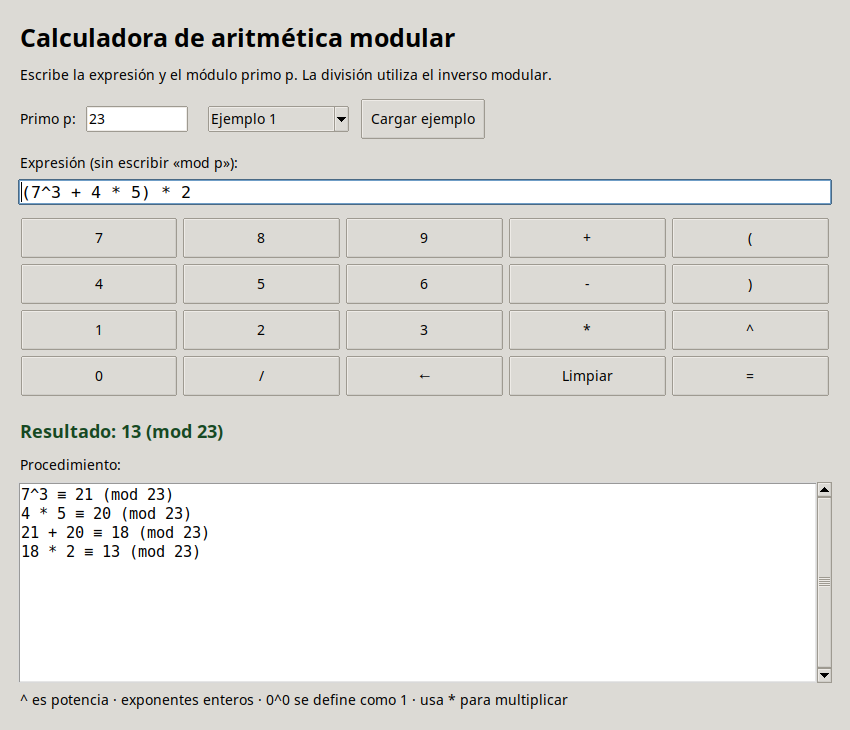
\includegraphics[width=0.82\textwidth]{capturas/ejemplo_1.png}\par
\small Figura 1. Ejecución real del ejemplo 1: resultado 13 módulo 23.
\end{center}

\newpage
\section*{3. Explicación del código: cálculo}
Todo el código de ejecución está en \texttt{calculadora.py}. Se separó el
cálculo matemático de los controles de la ventana para poder probar ambos.

\subsection*{3.1. Datos y validación del módulo}
\texttt{EJEMPLOS} guarda las cinco expresiones, sus módulos y los resultados
verificados. La función \texttt{es\_primo} descarta números menores que 2 y
pares distintos de 2; después busca divisores impares hasta la raíz cuadrada.
Si no existe ninguno, el número es primo. \texttt{calcular} valida que $p$
sea entero, primo y esté entre 2 y 1000000000.

\subsection*{3.2. Clase Analizador}
Esta clase transforma la expresión en un árbol: cada operación guarda sus
operandos y cada número se representa como un valor entero. No se utiliza
\texttt{eval} ni \texttt{exec}; el texto del usuario nunca se ejecuta como
código Python.
\begin{itemize}
\item \texttt{\_\_init\_\_}: comprueba los caracteres permitidos y separa
números, operadores y paréntesis. Aplica límites de longitud.
\item \texttt{ver} consulta el siguiente elemento sin consumirlo;
\texttt{tomar} lo consume y avanza una posición.
\item \texttt{analizar} inicia el recorrido y comprueba que no queden
símbolos sin interpretar.
\item \texttt{suma} agrupa sumas/restas y \texttt{producto} agrupa
multiplicaciones/divisiones, respetando su prioridad.
\item \texttt{signo} interpreta los signos positivos y negativos delante
de un número o de una expresión.
\item \texttt{potencia} reconoce \texttt{\^{}} y agrupa cadenas de potencias
a la derecha. Así, \texttt{2\^{}3\^{}2} significa $2^{(3^2)}$.
\item \texttt{atomo} reconoce enteros o expresiones entre paréntesis,
comprueba su cierre y rechaza posiciones incorrectas.
\end{itemize}

\subsection*{3.3. Exponentes: función entero}
El exponente se interpreta como un entero, no como un residuo módulo $p$.
Por ejemplo, en $2^{3+4}$ módulo $5$ se usa el exponente $7$ y se obtiene $3$;
reducir primero el exponente módulo $5$ daría un resultado incorrecto.
La función permite sumas, restas, productos, divisiones exactas y potencias
internas no negativas. Una división no exacta dentro del exponente se rechaza.

\subsection*{3.4. Función calcular y evaluador interno}
\texttt{calcular} valida el módulo, construye el árbol y llama a
\texttt{evaluar}. Esta función recorre primero los operandos y luego aplica
la operación. Los enteros y los resultados se reducen módulo $p$.
Para dividir se comprueba primero que el denominador no sea cero módulo $p$;
su inverso se obtiene con \texttt{pow(b, -1, p)}. Para una potencia se utiliza
\texttt{pow(a, exponente, p)}. Se devuelve el resultado junto con la lista de
pasos, incluyendo los inversos utilizados.

\newpage
\section*{4. Explicación del código: interfaz y controles}
\subsection*{4.1. Clase Calculadora}
\begin{itemize}
\item \texttt{\_\_init\_\_} crea la ventana, campos, selector de ejemplos,
teclado, resultado y área desplazable de procedimiento. Vincula Enter al cálculo.
\item \texttt{cargar} copia la expresión y el módulo del ejemplo elegido.
No calcula hasta pulsar el botón correspondiente.
\item \texttt{insertar} escribe el símbolo del botón en la posición del
cursor. Si hay una selección, la reemplaza. La flecha elimina la selección
o el carácter anterior.
\item \texttt{limpiar} borra expresión, resultado previo y procedimiento,
manteniendo el valor del módulo para la siguiente consulta.
\item \texttt{texto\_pasos} actualiza el área de explicación y la vuelve a
poner en modo de lectura para que no se altere el registro mostrado.
\item \texttt{resolver} convierte el módulo a entero, llama a
\texttt{calcular} y muestra el resultado. Captura errores de entrada y
expresiones demasiado anidadas; no cierra la ventana ante esos errores.
\end{itemize}
La función \texttt{main} abre la ventana de Tkinter y mantiene activo su ciclo
de eventos. La condición final \texttt{if \_\_name\_\_ == '\_\_main\_\_'}
permite ejecutar la ventana al abrir el archivo e importar las funciones para
las pruebas sin abrirla automáticamente.

\subsection*{4.2. Convenciones y límites}
Los signos negativos están permitidos: $-2^2$ significa $-(2^2)$, mientras
que $(-2)^2$ eleva al cuadrado el número negativo. Se define $0^0=1$, como
convención explícita de la calculadora. Una potencia negativa de cero es un error.

Se admiten hasta 500 caracteres, 200 elementos y 100 cifras por entero.
Los exponentes y sus cálculos intermedios están entre $-1000000$ y $1000000$.
Las potencias dentro de un exponente tienen además un límite de exponente
1000 y una cota de tamaño para evitar operaciones demasiado grandes. No se
admiten decimales, nombres de variables, multiplicación implícita ni llamadas
a funciones. Estos límites mantienen manejables las consultas de la interfaz.

\section*{5. Resultados y comprobación de los ejemplos}
Los cinco ejemplos se ejecutaron en el motor matemático y en la ventana.
Se obtuvieron, en el orden de la tarea, los resultados
\textbf{13, 10, 30, 25 y 37}. Los valores esperados se comprobaron también
con fracciones exactas y una búsqueda independiente del inverso.
\begin{center}
\begin{tabular}{c|r|r|r}
Ejemplo & Primo $p$ & Esperado & Obtenido \\
\hline
1 & 23 & 13 & 13 \\
2 & 29 & 10 & 10 \\
3 & 31 & 30 & 30 \\
4 & 37 & 25 & 25 \\
5 & 41 & 37 & 37
\end{tabular}
\end{center}

\newpage
\section*{6. Capturas reales y cálculo verificado}
Las imágenes se capturaron de la aplicación Tkinter en ejecución, en una
pantalla virtual aislada. No son diseños ni resultados simulados.
\begin{center}
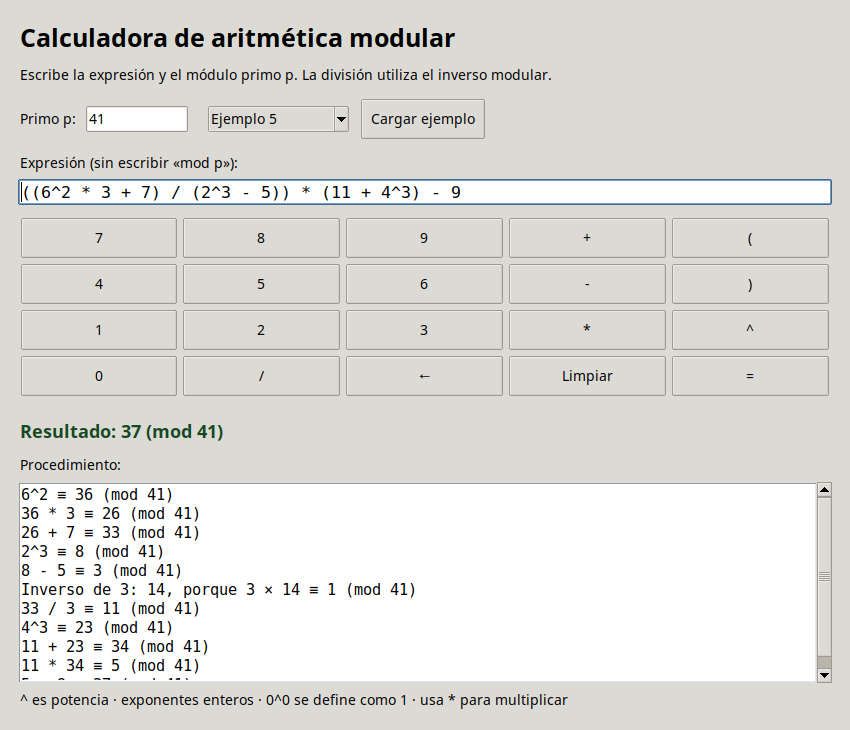
\includegraphics[width=0.65\textwidth]{capturas/ejemplo_5.png}\par
\small Figura 2. Ejemplo 5: resultado 37 módulo 41.
\end{center}
En este ejemplo, $6^2\cdot3+7\equiv33$ y $2^3-5\equiv3$ módulo $41$.
El inverso de $3$ es $14$, por lo que $33/3\equiv11$.
Además, $11+4^3\equiv34$. Finalmente,
$11\cdot34-9\equiv37\pmod{41}$.
\begin{center}
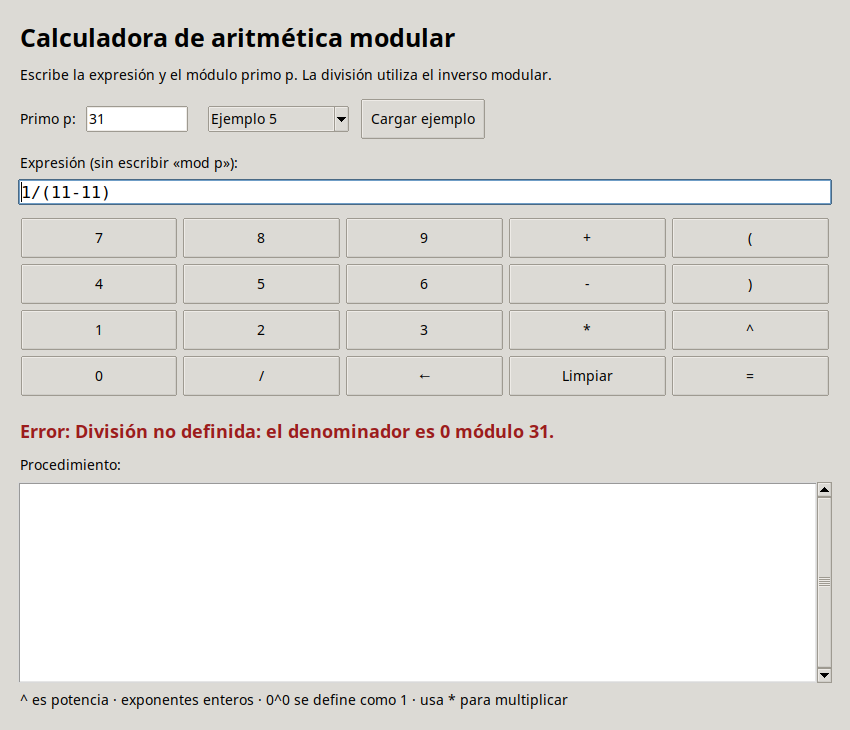
\includegraphics[width=0.65\textwidth]{capturas/error_division.png}\par
\small Figura 3. Rechazo de una división cuyo denominador es cero módulo 31.
\end{center}
La ventana informa el error y permite cambiar la expresión y volver a calcular.

\newpage
\section*{7. Pruebas de precisión y funcionamiento}
Se ejecutaron seis pruebas automatizadas con resultado correcto, incluida una
prueba de la ventana real. El registro se conserva en \texttt{pruebas.txt}.
\begin{itemize}
\item Los cinco ejemplos completos se compararon con sus resultados esperados.
\item Se comprobaron suma, resta, multiplicación, división y potencias para
los primos 2, 3, 5, 7, 11, 23, 29, 31, 37, 41 y 97, incluyendo valores negativos.
\item Se contrastaron los ejemplos con fracciones exactas, reduciendo el
resultado mediante un inverso encontrado por búsqueda, distinto del método del motor.
\item Se probaron prioridad de operadores, potencias encadenadas,
exponentes negativos, exponentes entre paréntesis y divisiones exactas en exponentes.
\item Se rechazaron módulos compuestos, paréntesis incompletos, caracteres
no permitidos y denominadores nulos incluso cuando su valor original no es cero:
por ejemplo, $1/7$ módulo $7$.
\item En la GUI se cargaron y calcularon los cinco ejemplos, se mostraron
errores, se limpió la entrada y se construyó una expresión usando los botones.
\end{itemize}
Para repetir las pruebas desde la carpeta del proyecto, con una sesión gráfica:
\begin{verbatim}
python3 -m unittest discover -s tests -v
\end{verbatim}
La prueba de la GUI requiere una pantalla disponible. En Linux sin escritorio
puede utilizarse Xvfb, como se describe en el README. El resultado registrado fue:
\begin{verbatim}
Ran 6 tests
OK
\end{verbatim}

\section*{8. Desafíos encontrados y soluciones}
\textbf{División modular.} La división ordinaria produce decimales y no
resuelve la operación en este sistema. Se sustituyó por el inverso modular
y se añadió una comprobación del denominador después de reducirlo.

\textbf{Prioridad y exponentes.} Interpretar \texttt{\^{}} como una operación
bit a bit o reducir el exponente como cualquier operando daría resultados
incorrectos. Se creó un analizador propio y una evaluación entera separada
para exponentes; las pruebas cubren ambas decisiones.

\textbf{Validación del código asistido por LLM.} Una expectativa inicial de
prueba del ejemplo 5 indicaba 30. La comprobación independiente mostró que
la respuesta correcta es 37; se corrigió esa expectativa. Este hallazgo
confirmó la necesidad de contrastar las respuestas generadas.

\textbf{Capturas y errores de interfaz.} Se utilizó una pantalla virtual para
probar la ventana y capturarla. Los errores de entrada se muestran dentro de
la aplicación, sin finalizar el programa.

\newpage
\section*{9. Conclusiones y aprendizajes}
La calculadora cumple las seis operaciones solicitadas y permite combinarlas
en expresiones con paréntesis. Los cinco ejemplos coincidieron con cálculos
independientes y la interfaz mostró los mismos resultados que el motor.

La principal diferencia frente a una calculadora ordinaria es la división:
solo se puede dividir por un residuo no nulo y se utiliza su inverso modular.
Exigir un módulo primo asegura que todo residuo no nulo tenga ese inverso.

Separar la interpretación de la expresión, el cálculo y la interfaz facilitó
localizar errores y probar cada parte. También se aprendió que los exponentes
requieren su propia interpretación entera y que los mensajes de error deben
explicar al usuario cómo corregir la consulta.

El uso de un LLM facilitó la generación del código y la documentación, pero
las pruebas matemáticas y de interfaz fueron necesarias para validar sus
propuestas. Los resultados se limitan al dominio y a las convenciones
expresamente documentados; no se presenta como un sistema de álgebra general.

\section*{Referencias}
Rosen, K. H. (2019). \textit{Discrete Mathematics and Its Applications}
(8.\textsuperscript{a} ed.). McGraw-Hill Education. Sección 4.1: divisibilidad
y aritmética modular; sección 4.4: resolución de congruencias.

Python Software Foundation. \textit{Built-in Functions}, función
\texttt{pow}: potencia modular e inversos.\par
\url{https://docs.python.org/3/library/functions.html#pow}

Python Software Foundation. \textit{tkinter: Python interface to Tcl/Tk}.\par
\url{https://docs.python.org/3/library/tkinter.html}

\section*{Archivos de la entrega}
\begin{itemize}
\item \texttt{calculadora.py}: programa completo y autónomo.
\item \texttt{documentacion/informe.tex}: fuente de este documento.
\item \texttt{documentacion/informe.pdf}: PDF compilado y revisado.
\end{itemize}
La carpeta \texttt{documentacion/capturas/} debe conservarse junto al TEX
para recompilarlo. El proyecto completo incluye estas imágenes y las pruebas.
\end{document}
